
\newcommand{\baselineCosImpls}{16~}
\newcommand{\baselineCosUnique}{4~}
\newcommand{\baselineCosUniqueIds}{2~}

\newcommand{\enumoCosImpls}{8~}
\newcommand{\enumoCosUnique}{5~}
\newcommand{\enumoCosUniqueIds}{3~}

\paragraph*{Megalibm.}
Next, we show how the
  ruleset inferred using \enumo for \herbie
  is also useful for
  Megalibm~\citep{megalibm}, another \eqsat
  tool that relies on numeric rewrites.
Given a transcendental operator,
  e.g., $\cos$,
  Megalibm synthesizes a set of low-level implementations
  that make different speed vs.\ accuracy tradeoffs.
A core phase in Megalibm
  is using \eqsat to discover various
  identities over such operators.

Using sound rules from
  rational, trig, and exponential \enumo programs (\autoref{table:herbie}),
  we ran the Megalibm benchmarks for $\sin$, $\cos$, and $\tan$.
Compared to Megalibm's manually developed ruleset,
  \enumo's rules would ideally discover
  at least as many \textit{unique} identities, in turn
  hopefully yielding as many or more \textit{unique}
  implementations across the speed vs.\ accuracy tradeoff space.

We detail the results for $\cos$ where
  the Megalibm baseline found the following identities:
  $\cos(x) = \cos(x + 4\pi)$,
  $\cos(x) = \cos(x + \pi + \pi)$,
  $\cos(x) = 2\cdot2\cdot \cos(-x) ~/~ 4$, and
  $\cos(x) = (\pi+\pi) - ((\pi+\pi) - \cos(-x))$.
The third and fourth identities are equivalent:
  both can be simplified to $\cos(x) = \cos(-x)$.
Similarly, the first identity
  is just two applications of the second.
Thus, the baseline only yielded 2 unique identities,
  from which Megalibm generated
  \baselineCosUnique implementations
  with differing speed and accuracy.
With \enumo-generated rewrite rules,
  Megalibm produces the following identities:
  $\cos(x) = \cos(x + (\pi + \pi))$,
  $\cos(x) = \cos(-x) \cdot 2 / 2$,
  $\cos(x) = \cos(\pi - x) - (\cos(\pi - x) \cdot 2)$,
  $\cos(x) = \cos(\pi - x) \cdot (- (\cos(\pi - x))^0)$, and
  $\cos(x) = -\cos(\pi - x)$.
Here, the third, fourth, and fifth identities are equivalent,
  yielding \enumoCosUniqueIds unique identities,
  which Megalibm used to find \enumoCosUnique unique implementations.
For $\tan$, Megalibm was able to use
  \enumo-generated rules to find
  \textit{new} identities of $\tan$
  where the baseline ruleset did not derive any.

\autoref{fig:megalibm-results} shows
  Megalibm's estimates of the speed vs.\ accuracy
  tradeoffs for implementations of $\cos$ generated by
  the \enumo-generated and manually developed baseline rulesets.
The table summarizes how,
  across $\sin$, $\cos$, and $\tan$,
  rules from \enumo always produced
  more unique identities,
  which typically also led to more unique implementations---except
  $\sin$, where
  the baseline yielded two extra implementations.
\enumo's rulesets
  can be applied across different tools in
  related domains and perform similarly to or better
  than manually developed expert rulesets.

\begin{figure}[t!]
  \centering
  \begin{subfigure}[T]{0.41\linewidth}
  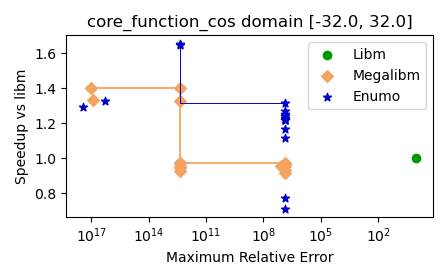
\includegraphics[width=\linewidth]{fig/megalibm/cos-3-pareto.png}
  \label{fig:megalibm-impls}
\end{subfigure}
  \hfill
  \begin{subfigure}[T]{0.58\linewidth}
    \centering
    \vspace{2em}
    \footnotesize
  \begin{tabular}{ccccc}
    \multirow{2}{*}{Fn} & \multicolumn{2}{c}{Megalibm} & \multicolumn{2}{c}{\enumo} \\ \cline{2-5}
    & \multicolumn{1}{c}{Unique Impls} & Unique Ids & \multicolumn{1}{c}{Unique Impls} & Unique Ids \\ \hline
    sin & \multicolumn{1}{c}{7} & 2 & \multicolumn{1}{c}{5} & 3 \\
    cos & \multicolumn{1}{c}{4} & 2 & \multicolumn{1}{c}{5} & 3 \\
    tan & \multicolumn{1}{c}{\color{red}{0}} & \color{red}{0} & \multicolumn{1}{c}{3} & 1  \\
    \end{tabular}
\end{subfigure}
  \caption{Megalibm analysis.
  (Left)
  The Pareto curve shows
    the implementations Megalibm found for
    cosine over the interval [-32.0, 32.0], with
  results normalized to the GNU libm implementations.
  Points up and to the right are better (faster and less error).
  Uniqueness is judged by clusters of performance.
  (Right)
  The number of unique identities and
    implementations generated with Megalibm's original rules
    and \enumo-synthesized rules.
  Notably,
    Megalibm found no identities or implementations for
    $\tan$, but \enumo did.
  }%
  \label{fig:megalibm-results}
\end{figure}

